
\chapter{Architecture}

This chapter contains an overview over the architecture for the system.
The first part will describe different views of the system and the
second part will show the quality attributes and patterns used when
developing the system.




The main parts of the system is shown in Figure~\ref{fig:systemOverview}. Clients sends
requests to the web server and receives the processed results. The
execution nodes process user submissions, and updates the results to
the database. 
\begin{figure}[t]
    \centering
 	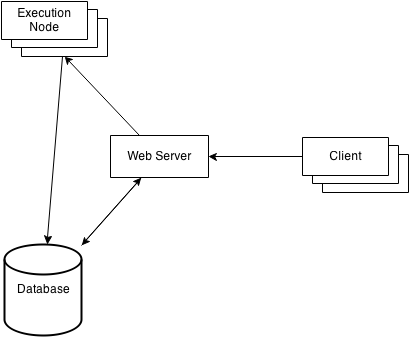
\includegraphics[scale=.5]{chapter06-img1.png} 
 	\caption{System overview}
 	\label{fig:systemOverview}
\end{figure}

\section{Views}

We have chosen to depict the architecture using Philippe
Kruchten's 4+1 view model. [1] This is a method of
describing the architecture for software-intensive systems from the
viewpoint of different stakeholder by using multiple, concurrent views.
We chose this model because it gives a good overview and is widely
accepted by the software industry. Below are the 4 main views in the
model; Logic, Process, Development, and Physical. The
``+1'' view is Use Cases which is
addressed in [Chapter 2 Task Description and Overview]

\subsection{Logic View}
The logical view describes the functionality of the system by breaking
down requirements into classes and representing them, and their
relations, through class and sequence diagrams.
\begin{figure}[h!]
    \centering
	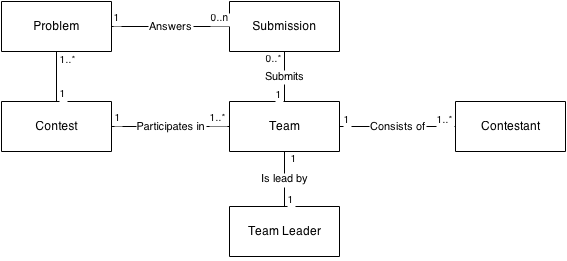
\includegraphics[scale=.5]{chapter06-img2.png} 
	\caption{Top level class diagram}
\end{figure}

Figure 6.1 shows the main classes involved in GentleIDI.\ Each team
participates in a single contest, and consists of a predefined number
of contestants. Each team also has a team leader that handles most of
the administrative tasks. The team can also try to solve problems by
uploading submissions. 

\subsection{Process View}
The process view explains the communication between different processes
in the system, as well as how the system behaves in runtime. 

As this system is a web application the first thing to note is that
there will be concurrent users in runtime. Each user generates HTTP
requests to the server, which in turn may execute database lookups for
information like score tables or problem sets. When a user submits a
solution the system will place it in a queue, which decides which node
the solution will execute on according to availability and load. 

We will now show examples for two important parts of the application.
First is the action of successfully registering a user and creating a
team. See figure~\ref{fig:actRegister}.
\begin{figure}[h!]
    \centering
	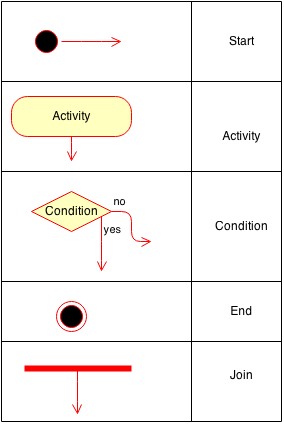
\includegraphics[scale=.5]{chapter06-img3.png} 
	\caption{Symbology}
\end{figure}

\begin{figure}[h]
	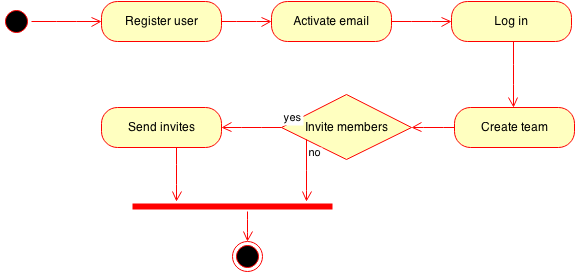
\includegraphics[width=0.8\textwidth]{chapter06-img4.png} 
	\caption{Activity Diagram for registering a user and a team}
	\label{fig:actRegister}
\end{figure}

Second is submitting a solution to a programming problem. See figure~\ref{fig:actSubmit}.
\begin{figure}[h]
	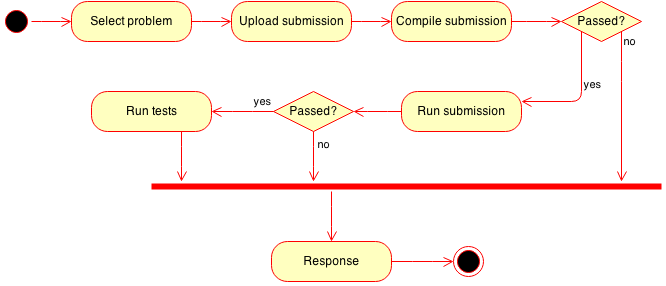
\includegraphics[width=0.8\textwidth]{chapter06-img5.png}
	\caption{Activity Diagram for submittion a solution}
	\label{fig:actSubmit}
\end{figure}

\subsection{Development View}
\subsubsection{Purpose}

The developer view is intended for the developers. It should ease
development, and focus on software module organization by packaging the
software in small chunks.

We wanted a modular and maintainable system where it is easy to maintain
and change specific parts of the system without changing everything.
The structure of the system can therefore be divided into the following
main packages: Contest, Registration, Submission, Execution, Balloon,
Clarification, Admin, and Article. These packages are described in
detail in chapter 8 Implementation. 

\subsection{Physical View}
\label{sec:physicalView}

\subsubsection{Purpose}
The physical view shows the interaction between the physical components
of the system.

Physically the system is structured as a multitiered architecture. It
consists of three tires, presentation tier, application tier, and data
tier, see figure~\ref{fig:multitier}. The tiers represents a physical
structuring mechanism for the system infrastructure. The user is physically
separate from the application and database. 

\begin{figure}[h]
	\centering
	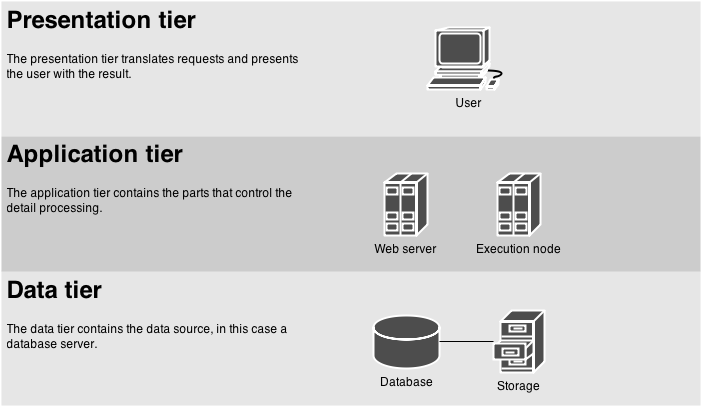
\includegraphics[width=0.8\textwidth]{chapter06-img6.png}
	\caption{Multitier architecture}
	\label{fig:multitier}
\end{figure}
\subsubsection{Presentation tier}

This tier presents information to the user through the public website
and admin interface. It translates the web server response into web
pages generated using HTML5, CSS, Ajax, and JavaScript. It sends
requests to the underlying web server and renders the response.

\subsubsection{Application tier}\label{section:applicationTier}

The application tier contains the logical layer, it controls an
application's functionality by performing detailed
processing. Primarily this is done through python code, although when
running solutions the file is run on an execution node through the use
of built in unix commands. 

This splits the application tier in two parts, the web server that
serves static and dynamic content, and the execution nodes that process
uploaded submissions. This division can be seen in
``Application Tier'' in Figure~\ref{fig:multitier}.


For the web server we use Nginx for serving static files, and as a
reverse proxy for Gunicorn, the server providing dynamic HTTP content
to the user. Gunicorn is the server that processes requests and returns
HTTP pages. The execution nodes process submissions through a FIFO
queue implemented with Celery and RabbitMQ.\ This provides load
balancing across CPU cores and multiple nodes in the cluster. The
execution nodes also share parts of the filesystem, this is implemented
with SSHFS (SSH Filesystem), and is a secure way of sharing the
uploaded files across the execution nodes. 


\subsubsection{Data tier}

This tier includes the data control functionality. The system utilises a
shared SQL database for the execution nodes and the web server. See
Figure~\ref{fig:systemOverview}. This database links to the file storage on the main web
server. However, the execution nodes requires some files to be shared
across multiple nodes. Like explained earlier in
section~\ref{section:applicationTier}, this is implemented with SSHFS.\ For
more specific details see~\ref{chapter:implementation} and~\ref{appendix:ER}.


\section{Quality attributes}

\subsection{Availability}

Since this software is to be used in a programming contest, it is
crucial that the system has high uptime and availability. And since the
contest only lasts for about 4 hours, our margin for failure is
minimal. We have made an effort to account for all possible outcomes,
and to safeguard the application for any errors that might occur. 

\subsection{Modifiability}

This is a system that we hope will be used for many years to come. With
the ever changing nature of the web, the ability to adapt and improve
is imperative. To accommodate this, we chose to implement our solution
in Python, a language taught to most of new students of computer
courses at NTNU.\ These are the same students that hopefully will use
and continue to work on this software. To our best ability we have also
tried to write and document the code in a way such that it is easy to
understand and improve.

\subsection{Performance}

Performance is an important aspect of every application, especially web
applications. Users expect that sites loads fast. Failing to accomplish
this is a sign of a bad application, at least from the
user's perspective. For this reason we have focused on
making our pages load as fast as possible. And since this application
will be used by over 100 users simultaneously, it is also important
that the servers will handle the load. \ 

\subsection{Security}

Since our application contains user data and data that should be hidden
from unauthenticated users, security is another important aspect.
Django provides many security features by default, and others that can
be implemented with very little effort. We also chose to enable SSL on
the web server to increase security on web requests.

\subsection{Testability}

When we first started out, we wanted to utilize testing during
development. Testing is a way to find problems early, and before they
begin to encompass larger parts of the application. But testing is also
one of the most time consuming parts of the development process. In the
end we did not have as much test coverage as we would like, but we feel
that we covered the most important parts.

\subsection{Usability}

As with any web application, we want the users of the system to
accomplish their desired task, and learn the functions of the system
with ease. The user should receive feedback if something went wrong or
if the outcome is not clear. We also want the web pages to provide
information how to use the system. \ 

\section{Patterns}

\subsection{Client-Server}

Since we are making a web application we will use the Client-Server
pattern. The clients connect to the server through a web interface,
either the website or the admin interface. 

\subsection{MVC(model-view-controller)}

The front end is implemented using the Django framework and follows a
rather strict implementation of MVC.\ Every HTTP request sent to the
site is handled by a controller function, which in turn fetches the
appropriate models from a database, creates a view based on the models
and returns the view as an HTTP response. 

\subsection{Shared-Data}

The system utilises multiple execution nodes as well as a web server,
through which users access data. We wanted to have a central shared
database server that scales with the number of execution nodes and the
amount of data. 

\subsection{Multi-tier}

See:~\ref{sec:physicalView} Physical View.
References:

[1] Architectural Views -
% http://www.cs.ubc.ca/\~{}gregor/teaching/papers/4+1view-architecture.pdf

